%% ----------------------------------------------------------------
%% Introduction.tex
%% ---------------------------------------------------------------- 
\chapter{Introduction} \label{Chapter:Introduction}
%The Introduction to my Report \dots

%The initial idea of the project was taken from Pirobot(\cite{Pirobot}).
%
%\inote{what it will do. Define everything. Use. Very general}
%General - mapping robots. 
%
%stereovision - uses etc.
%
%other similar projects
%
%why mine is important 


This report documents the design, testing and building of a stereoscopic mapping robot. The end product will be a small, two wheeled robot with a roller ball, that will autonomously search and map an unknown area and produce an occupancy map of the searched area. 

An occupancy map is a representation of an area where a location is given a value of either \textit{free, occupied} or \textit{unkown} (\cite{thrun2003learning}).  Three dimensional occupancy maps can also be generated, such as the OctoMap (\cite{octomap}). Objects can also be tracked using an occupancy map and statistics (\cite{Fleuret:OccupancyMap}). 

The purpose of a mapping robot is to build a representation of the area around it. This then facilitates the use of any application that requires prior knowledge of the area. One algorithm that is used to build up an occupancy map is the S.L.A.M. algorithm (\cite{Thrun:SLAM}) and is used in other mapping robots(\cite{Se:MappingRobot}). Accurate mapping robots tend to use laser range finders (\cite{Ruhnke:LaserMapping}).

Stereoscopy in computer vision is the ability to calculate the locations and depths using images from two or more cameras, which are used to triangulate and estimate distances (\cite{Saxena:DepthEstimation}). By using two cameras on the same plane, separated by a set horizontal distance, the depth of the observed scene can be perceived by the system.

Stereovision is a small section of computer vision which is widely used in many applications, including Microsoft's Xbox Kinect (\cite{Microsoft:Kinect}), where stereo vision is used to locate a game player in order to use their movements to control the game. \cite{Mrovlje:Distance_Stereoscopic} uses stereovision to be able to locate the distance to a marker.

The stereovision mapping robot discussed in this report is a low cost alternative to other robots which use laser range finders or high quality cameras (\cite{Se:MappingRobot}). The robot will use the base seen in figure \ref{fig:RobotBase} and use two OmniVision OV7670 cameras delivering QVGA format images.

\begin{figure}
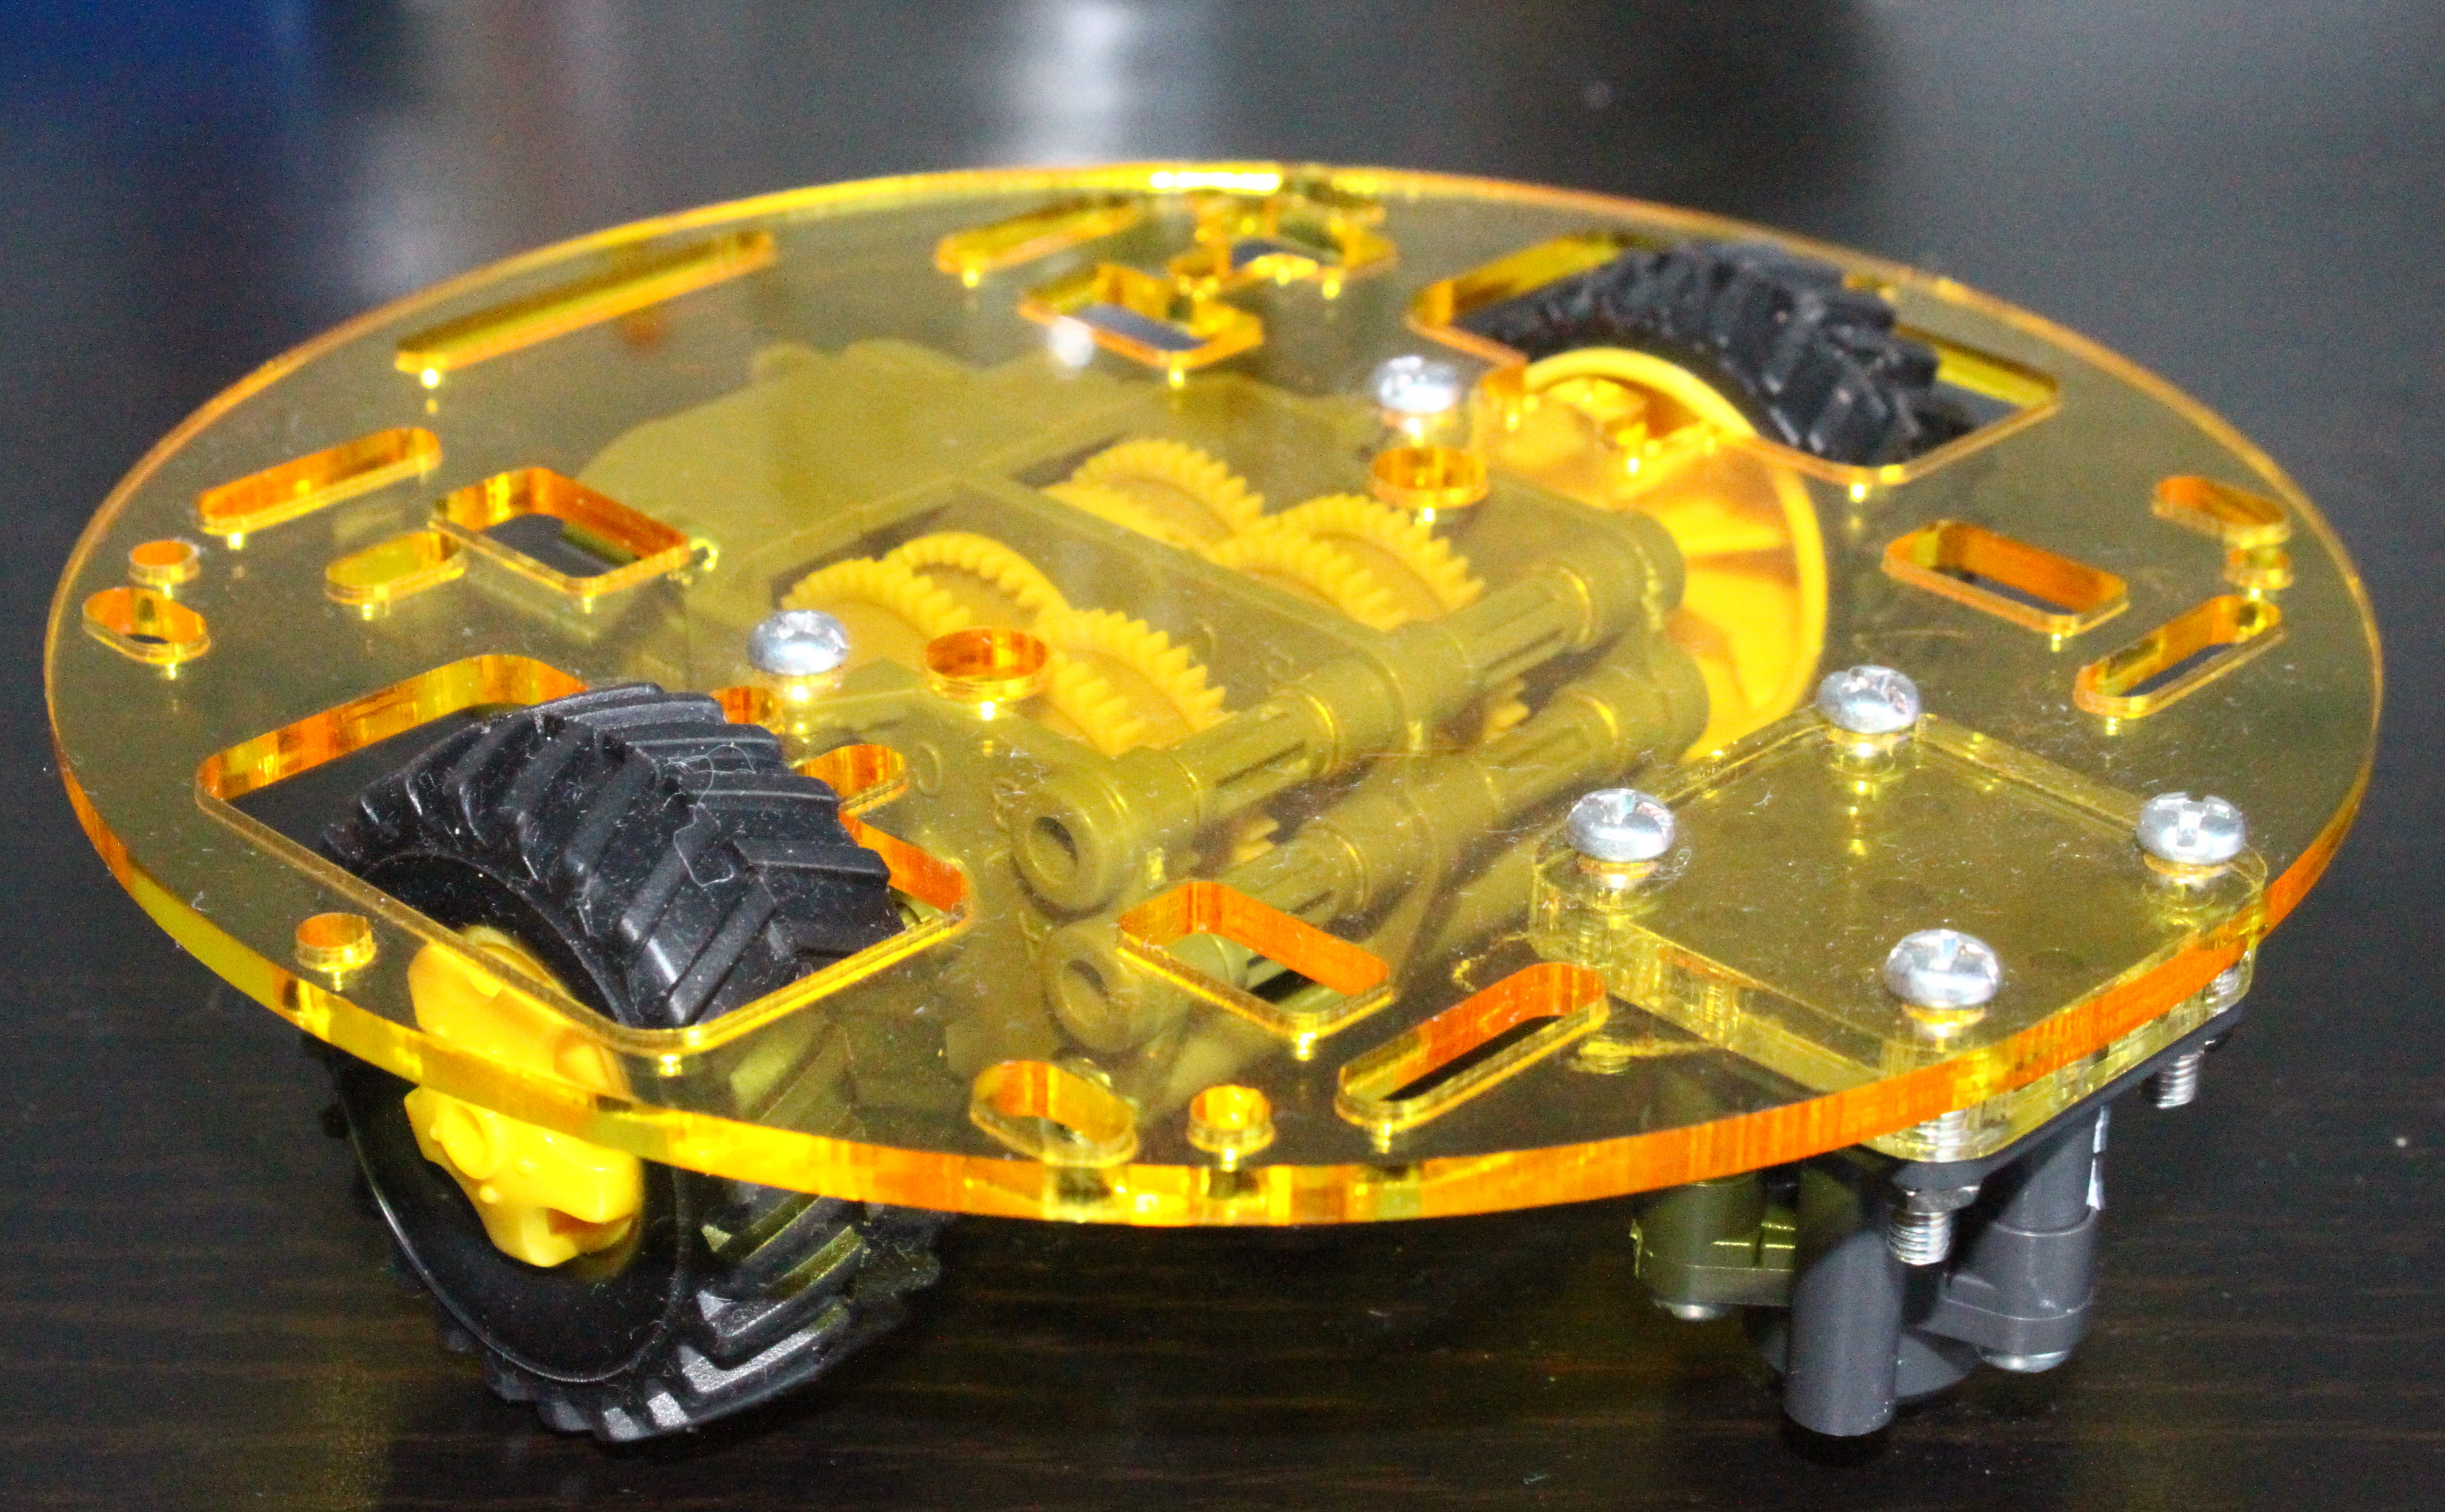
\includegraphics[width=\textwidth]{./Figures/RobotBase.jpg}
\caption{The base of the robot}
\label{fig:RobotBase}
\end{figure}

\section{Project Management}
In order to reduce the risk within the project, all aspects of potential issues are looked at and are summarised in table \ref{tab:risk}. A Gantt chart of how time will be spent can be seen in figure \ref{fig:Gantt}. 

The project will be designed in stages - first, gaining operation of all the basic sections; movement, image capturing, image detection algorithms etc. These will then be brought together once tested to create the final product. 
\begin{table}
\begin{tabular}{|p{6cm}|p{2cm}|p{6cm}|}\hline
Risk						&	Severity	&	Prevention \\ \hline
Parts not arriving on time	&	High		&	Order parts as early as possible \\
Project not fulfilling specification				&	High		&	Develop in stages to obtain functionality in parts. Ensure enough time is allocated to the project.	\\
PCB Design is incorrect		&	Medium		&	Check the design carefully and get second opinion \\
Failure of personal computer causing data loss & Low	& 	Keep back ups of all work on Devtrack Git repository and Dropbox.\\

\hline
\end{tabular}
\caption{A list of risks and the prevention steps taken to reduce their impact}
\label{tab:risk}
\end{table}
